%----------------------------------------------------------------------------------------
%	Inställningar och dokumentkonfiguration
%----------------------------------------------------------------------------------------

\documentclass[paper=a4, fontsize=11pt]{report} % A4-sida och 11 punkters fontstorlek

\usepackage[T1]{fontenc} % 8-bitarskodning som har 256 glyfer
\usepackage[english]{babel} % Svenskt språk
\usepackage[utf8]{inputenc} % För svenska tecken
\usepackage{dtklogos} % Logos
\usepackage{wallpaper} % Bakgrundsbild
\usepackage{fancyhdr} % Specialsidhuvud och sidfot
\usepackage{enumerate} 
\usepackage{xifthen}% provides \isempty test
\usepackage{listings}% Code examples
\usepackage{xcolor}
\newcounter{tmpc}
\lstdefinestyle{BashInputStyle}{
  language=bash,
  basicstyle=\footnotesize\ttfamily,
  numbers=left,
  numberstyle=\tiny,
  numbersep=3pt,
  frame=tb,
  columns=fullflexible,
  backgroundcolor=\color{yellow!20},
  linewidth=0.9\linewidth,
  xleftmargin=0.1\linewidth
}
% Exampels
% Inline
% \lstinline[style=BashInputStyle]´# apt-get --purge remove rubygems´.
% Multiline
% \begin{lstlisting}[style=BashInputStyle]
%    # apt-get --purge remove rubygems
% \end{lstlisting}

\pagestyle{fancyplain} % Använd sidhuvud och sidfot på alla sidor
\fancyhead[L]{Seminar 5 -- 1DV020 -- 2015 -- Server Administration} % Titel till vänster i sidhuvud
\fancyhead[C]{} % Tomt i mitten
\fancyhead[R]{} % Tomt till höger
\fancyfoot[L]{} % Tomt till vänster
\fancyfoot[C]{} % Tomt i mitten
\fancyfoot[R]{\thepage} % Sidnumrering till höger i sidfoten
\renewcommand\thesection{\arabic{section}} % Section beter sig som i dokumentklassen article

\newcommand{\win}[1]{Microsoft Windows Server\ifthenelse{\isempty{#1}}{}{ #1}}
\newcommand{\gui}[0]{``Server with a GUI''}
\newcommand{\core}[0]{Windows Server Core}
%----------------------------------------------------------------------------------------
%	TITLE SECTION
%----------------------------------------------------------------------------------------
\newcommand\BackgroundPic{
    \put(-50,-50){
    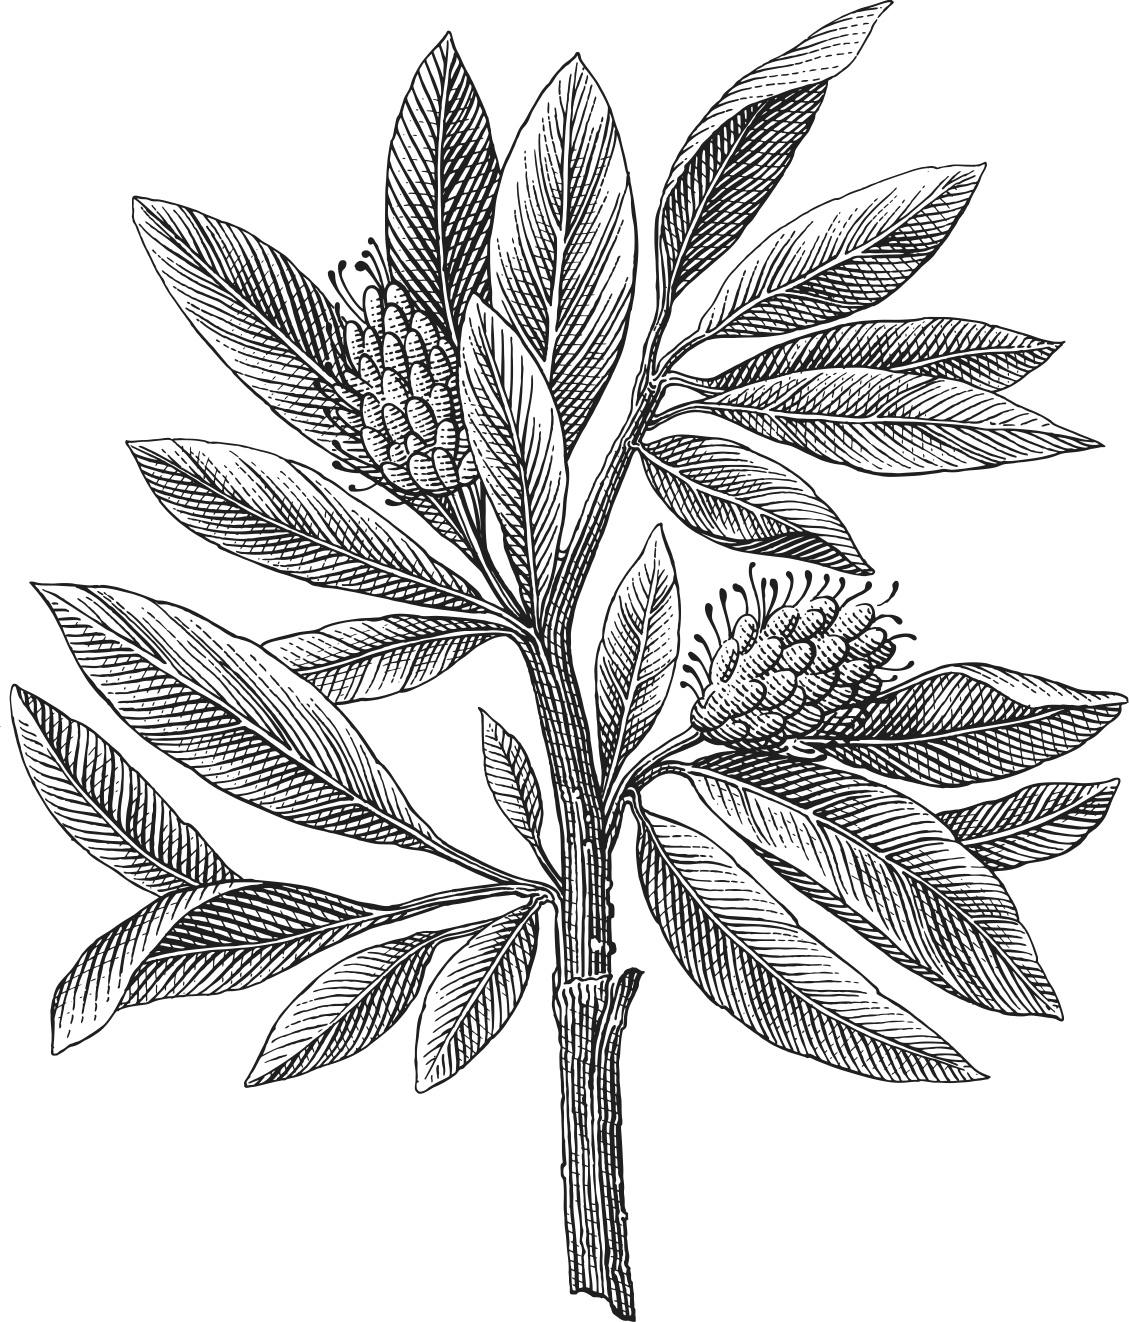
\includegraphics[keepaspectratio,scale=0.65]{lnu_etch.png} % Bakgrundsbild
    }
}
\newcommand\BackgroundPicLogo{
    \put(15,700){
    
\includegraphics[keepaspectratio,scale=0.10]{logo.png} % Logga i vänstra hörnet
    }
}

\newcommand{\horrule}[1]{\rule{\linewidth}{#1}} % Skapa hortisontell linje

\title{	\vspace{-10cm}
    \normalfont \normalsize
    \textsc{Linnaeus University} \\ [25pt] % Universitetes namn
    \horrule{0.5pt} \\[0.4cm] % Tunn linje högst upp
    \huge Seminar 5\\ % Arbetes titel
	\large \textcolor{gray}{1DV020 -- Server Administration}
    \horrule{0.5pt} \\[0.4cm] % Tunn linje längst ner
}

\author{Jacob Lindehoff} % Författarnas namn

\date{\normalsize\today} % Dagens datum

\begin{document}
\AddToShipoutPicture*{\BackgroundPic} % Lägger in backgrundsbild på första sidan
\AddToShipoutPicture*{\BackgroundPicLogo}
\maketitle % Skriv ut titeln
\noindent % Tabba inte in på första meningen


%------------------------------------------------
%	Introduktion
%------------------------------------------------
\section{Introduction}
During this seminar, we will address the following topics:
\begin{itemize}
	\item Backup
	\item Reliability
	\item Performance
	\item Troubleshooting
\end{itemize}

%------------------------------------------------
%	Deadline
%------------------------------------------------
\section{Deadline}
  The seminar is on the {\color{red}11th of March 2015} and it is compulsory. If you cannot participate, it must be notified in advance and a written report of the seminar must be submitted no later than {\color{red}3 days} after the seminar. The written report should contain detailed answers to all questions in the seminar.\newpage
%------------------------------------------------
%	Seminariefrågor
%------------------------------------------------
\section{Seminar Questions}
\begin{enumerate}
\begin{large}
\item Describe the following types of backup:
\begin{enumerate}[a.]
	\item Full or Normal backup
	\item Differential backup
	\item Incremental backup
\end{enumerate}
\item How does Windows Server Backup in Windows Server 2012 R2?
\item What is Volume Shadow Copy Service and how does it work?
\item What tools are integrated in Windows Server to handle troubleshooting and monitoring of the operating system?

\item A popular way to backup files in linux is using rsync Explain how it works.
\item Is the rsync traffic encrypted or in cleartext?
\item Give examples of some useful rsync commands.
\item What is rsnapshot? How does it work?
\item What would you need to do to automate rsync/rsnapshot?
\item What three reasons are there for providing a restore  and give one example for each of these?

\item Shortly explain these terms:
\begin{enumerate}[a.]
	\item Corporate guidelines
	\item SLA(Service Level Agreement)
	\item Policy
	\item Procedure
	\item Schedule
\end{enumerate}

\item Setting up a Backup-Schedule, what should you consider when determining:
\begin{enumerate}[a.]
	\item The cycle size?
	\item The time of backup?
\end{enumerate}

\item A company has a 2000 GB drive with an average daily change of 2\% and a 7 day cycle.
\begin{enumerate}[a.]
	\item Calculate the total amount of space that is required after 10 days.
	\item  Would you aruge there are any better or worse scopes?
\end{enumerate}
\item What three procedures in a backup can be automated?
\item Why is it so important to have “firedrills” on backups? And what considerations should you take when doing it?
\item What are the benefits and drawbacks from using an offsite/cloudbased backup solutions to an inhouse? Are there any certain consideration you should take in any of the implementations?
\item What are the advantages/disadvantages with diskbased and tapebased backups?
\item What is a Tape jukebox?
\item Read the chapter of debugging and relate to some of the debugging procedure that you have used/could’ve used?


\end{large}
\end{enumerate}
\end{document}
